\documentclass{article}

\usepackage{graphicx}
\usepackage{rotating}
\usepackage{amsmath}
\usepackage{amssymb}
\usepackage{fancyhdr}
\usepackage{listings}
%\usepackage{xcolor}
\usepackage{color}
\usepackage{amsfonts}
\usepackage{textcomp}
\usepackage{float}
\usepackage[sorting=none]{biblatex}
\usepackage[margin=1in]{geometry}
\usepackage[font={small,it}]{caption}
\usepackage[table,xcdraw]{xcolor}
\usepackage{placeins}
\usepackage{xepersian}





%\DeclareMathOperator*{\btie}{\bowtie}
\addbibresource{bibliography.bib}
\settextfont[Scale=1.2]{B-NAZANIN.TTF}
\setlatintextfont[Scale=1]{Times New Roman}
\renewcommand{\baselinestretch}{1.5}
\pagestyle{fancy}
\fancyhf{}
\rhead{تکلیف اول درس مبانی هوش محاسباتی}
\lhead{\thepage}
\rfoot{علیرضا ابره فروش}
\lfoot{9816603}
\renewcommand{\headrulewidth}{1pt}
\renewcommand{\footrulewidth}{1pt}
%%%%%%%%%%
\lstset
{
    language=[latex]tex,
    basicstyle=\ttfamily,
    commentstyle=\color{black},
    columns=fullflexible,
    keepspaces=true,
    upquote=true,
    showstringspaces=false,
    morestring=[s]\\\%,
    stringstyle=\color{black},
}
%%%%%%%%%%
%beginMatlab
\definecolor{mygreen}{RGB}{28,172,0} % color values Red, Green, Blue
\definecolor{mylilas}{RGB}{170,55,241}
%endMatlab
\begin{document}
%beginMatlab
\lstset{language=Matlab,%
    %basicstyle=\color{red},
    breaklines=true,%
    morekeywords={matlab2tikz},
    keywordstyle=\color{blue},%
    morekeywords=[2]{1}, keywordstyle=[2]{\color{black}},
    identifierstyle=\color{black},%
    stringstyle=\color{mylilas},
    commentstyle=\color{mygreen},%
    showstringspaces=false,%without this there will be a symbol in the places where there is a space
    numbers=left,%
    numberstyle={\tiny \color{black}},% size of the numbers
    numbersep=9pt, % this defines how far the numbers are from the text
    emph=[1]{for,end,break},emphstyle=[1]\color{red}, %some words to emphasise
    %emph=[2]{word1,word2}, emphstyle=[2]{style},    
}
%endMatlab
\begin{titlepage}
\begin{center}

\includegraphics[width=0.4\textwidth]{figures/IUT Logo.png}\\
        
\LARGE
\textbf{دانشگاه صنعتی اصفهان}\\
\textbf{دانشکده مهندسی برق و کامپیوتر}\\
        
\vfill
        
\huge
\textbf{عنوان: تکلیف چهارم درس ریزپردازنده}\\
        
\vfill
        
\LARGE
\textbf{نام و نام خانوادگی: علیرضا ابره فروش}\\
\textbf{شماره دانشجویی: 9816603}\\
\textbf{نیم\,سال تحصیلی: پاییز 1400}\\
\textbf{مدرّس: دکتر عارف کریمی افشار}\\
\end{center}
\end{titlepage}


%\tableofcontents
\newpage


\section{}%1
\subsection{نتیجه (خروجی)}

یک مدل رگرسیون خطی مبتنی بر یک متغیر وابسته پیوسته است. این به معنای این است که متغیر وابسته مقادیر عددی را به جای دسته‌بندی زیرمجموعه‌ها یا گروه‌ها پذیرفته می‌کند. در مقابل، مدل‌های رگرسیون لجستیک مبتنی بر متغیرهای وابسته دودویی هستند. متغیر وابسته فقط می‌تواند دو مقدار 0 یا 1 را بپذیرد. همچنین، خروجی رگرسیون خطی مقدار پیوسته دارد (محدوده‌ای از مقادیر را برمی‌گرداند). برای مثال،
\begin{itemize}
	\item طول سقف (25 اینچ، 19 اینچ، 5 فوت)
	\item ارتفاع (5 فوت و 8 اینچ، 6 فوت و 2 اینچ، 5 فوت و 10 اینچ)
	\item سرعت فرار (26000 مایل در ساعت، 21500 مایل در ساعت، 29500 مایل در ساعت)
\end{itemize}
در عین حال، مدل رگرسیون لجستیک بیان احتمالاتی دارد. به عنوان مثال:
\begin{itemize}
  \item احتمال شکست در یک بازی تنیس 84.3 درصد است
  \item احتمال تصویب یک قانون در کنگره 23.1 درصد است
  \item احتمال اعمال محدودیت شبانه‌روزی در زمان شیوع کروناویروس 65.1 درصد است
\end{itemize}
علاوه بر این، رگرسیون خطی توزیع نرمال یا گاوسی را مشاهده می‌کند و رگرسیون لجستیک توزیع دوجمله‌ای را نشان می‌دهد.

\subsection{ارتباط بین متغیرها}

فهم رابطه بین متغیرها در هنگام تصمیم‌گیری درباره نوع مدل رگرسیون برای اهداف مختلف بسیار حائز اهمیت است.

رگرسیون خطی یک رابطه خطی بین متغیرها را با رسم یک خط راست بر روی نمودار توصیف می‌کند. این امکان را به حرفه‌ای‌ها می‌دهد تا روابط خطی را بررسی کرده و حرکت آن‌ها را در طول زمان پیگیری کنند. در مقابل، رگرسیون لجستیک برای مطالعه و بررسی احتمال وقوع یک رویداد شناخته شده است. از آنجا که ساختار خطی رابطه متغیری را نشان نمی‌دهد، پیگیری رگرسیون لجستیک با استفاده از ساختارهای خطی لازم نیست.

\subsection{خطا}
هدف رگرسیون خطی یافتن بهترین خط تطبیق داده شده است در حالی که رگرسیون لجستیک مقادیر خط را به منحنی سیگموید متناسب می‌کند. روش محاسبه‌ی تابع خطای رگرسیون خطی، خطای میانگین مربعات است، در حالی که برای رگرسیون لجستیک، این مقدار با استفاده از تخمین بیشینه درست‌نمایی محاسبه می‌شود. رگرسیون خطی از خطای میانگین مربعات (\lr{RMSE}) برای محاسبه مقدار وزن بعدی نقاط داده‌ای (یا مشاهدات) از طول خط رگرسیون استفاده می‌کند. به عکس رگرسیون لجستیک از روش دقت برای پیش‌بینی مقدار وزن بعدی استفاده می‌کند.

\subsection{روش‌های تخمین (برآورد)}
یک مدل رگرسیون خطی از روش \lr{"ordinary least squares"} استفاده می‌کند تا بهترین رابطۀ رگرسیون را پیدا کند. با توجه به این روش، ضرایب رگرسیون برای کاهش جمع مربعات فاصلۀ هر متغیر پاسخ به مقدار سازگاری انتخاب می‌شوند.

در مقابل، رگرسیون لجستیک از روش \lr{"maximum likelihood estimation"} استفاده می‌کند، جایی که ضرایب رگرسیون برای بیشینه کردن احتمال $y$ به ازای یک مقدار $x$ داده شده (احتمال مطلوب) انتخاب می‌شوند. در زمینه یادگیری ماشین، سیستم با چند بار تکرار، مقادیر بیشینه‌ی احتمال را به دست می‌آورد.

یک مدل رگرسیون خطی با در نظر گرفتن مجموع مقادیر تمام ویژگی های ورودی (متغیرها)، یک خروجی $y$ (مقدار واقعی) را برآورد می‌کند.

مدل مقادیر ضرایب $z, p_1, p_2, p_3, \cdots , p_n$ را تعیین کرده و در نتیجه با کمترین خطا به داده‌های آموزشی سازگاری داده شده است تا خروجی واقعی ($y$) را پیش‌بینی کند.

از طرفی دیگر، مدل رگرسیون لجستیک با محاسبه‌ی مجموع مقادیر متغیرهای ورودی، یک تابع لجستیک یا سیگموید را در نتیجه اعمال می‌کند. به این ترتیب، تابع غیر خطی یک خروجی دودویی به شکل 0 یا 1 (یا حتی "صحیح یا غلط") در اختیار ما قرار می‌دهد.


\section{}%2
چندین دلیل وجود دارد که تابع هزینه‌ی میانگین مربعات خطا استفاده شده در رگرسیون خطی، برای رگرسیون لجستیک مناسب نیست:
\begin{enumerate}
	\item غیرخطی بودن تابع لجستیک: تابع لجستیک مورد استفاده در رگرسیون لجستیک، غیرخطی است؛ به این معنی که رابطه‌ی بین متغیرهای ورودی و احتمال خروجی یک خط نیست. تابع هزینه‌ی میانگین مربعات خطا رابطه‌ی خطی بین ورودی و خروجی را فرض می‌کند که برای رگرسیون لجستیک مناسب نیست.
	\item مقادیر خروجی احتمالات هستند: در رگرسیون لجستیک، مقادیر خروجی احتمالاتی هستند که بین 0 و 1 واقع می‌شوند. تابع هزینه‌ی میانگین مربعات خطا، مقادیر منفی را می‌تواند تولید کند، که احتمالات معنی داری ندارند.
	\item حساسیت به داده های پرت: تابع هزینه‌ی میانگین مربعات خطا، حساس به داده های پرت است که می تواند باعث ایجاد خطاهای بزرگ در تابع هزینه شود. در رگرسیون لجستیک، داده‌های پرت می‌توانند تأثیر قابل توجهی بر احتمالات حاصل شده داشته باشند، لذا استفاده از یک تابع هزینه‌ی کمتر حساس به داده‌های پرت مهم است.
	\item داده‌های نامتعادل: تابع هزینه‌ی میانگین مربعات خطا فرض می‌کند که داده‌ها متعادل هستند. به این معنی که تعداد مثبت و منفی مثال‌ها برابر است. با این حال، در کاربرد‌های واقعی، داده‌ها اغلب نامتعادل هستند که می‌تواند به پیش‌بینی‌های \lr{bias}شده منجر شود.
	\item محدب‌نبودن: تابع هزینه‌ی میانگین مربعات خطا، در رگرسیون خطی محدب است. اما در رگرسیون لجستیک محدب نیست. به این معنی که الگوریتم‌های بهینه‌سازی ممکن است در مینیمم‌های محلی گیر کنند و پیدا کردن مینیمم کلی تابع هزینه مشکل باشد.
\end{enumerate}
به همین دلیل، استفاده از تابع هزینه‌ای که به طور خاص برای رگرسیون لجستیک طراحی شده است، مانند تابع هزینه‌ی \lr{cross-entropy}، بهتر است. تابع هزینه‌ی  \lr{cross-entropy}، قادر به تشخیص رابطه‌ی غیرخطی بین متغیرهای ورودی و احتمالات خروجی است و کمتر حساس به داده‌های پرت است.


\section{}%3
از معادله‌ی اول شروع می‌کنیم:
\begin{latin}
$
p(X) = \frac{e ^ {\beta_0 + \beta_1 X}}{1 + e ^ {\beta_0 + \beta_1 X}} \Rightarrow \\
\frac{p(X)}{1 - p(X)} = \frac{\frac{e ^ {\beta_0 + \beta_1 X}}{1 + e ^ {\beta_0 + \beta_1 X}}}{1 - \frac{e ^ {\beta_0 + \beta_1 X}}{1 + e ^ {\beta_0 + \beta_1 X}}} =  \frac{\frac{e ^ {\beta_0 + \beta_1 X}}{1 + e ^ {\beta_0 + \beta_1 X}}}{\frac{1}{1 + e ^ {\beta_0 + \beta_1 X}}} = e ^ {\beta_0 + \beta_1 X} \Rightarrow \\
\ln\left( \frac{p(X)}{1 - p(X)} \right) = \beta_0 + \beta_1 X
$
\end{latin}
بنابراین، این دو معادله معادل هستند و رابطه‌ای مشابه بین متغیر وابسته و مستقل در رگرسیون لجستیک را توصیف می‌کنند. به عبارت ديگر، نمايش تابع لجستيك و نمايش لاجيت براي مدل رگرسيون لجستيك معادل هستند.


\section{}%4
رگرسیون لجستیک در اصل برای مسائل دسته‌بندی دو کلاسه طراحی شده است. با این حال، روش‌های متعددی برای گسترش رگرسیون لجستیک برای مسائل دسته‌بندی چند کلاسه وجود دارد که در آن متغیر وابسته می‌تواند بیش از دو مقدار ممکن داشته باشد.
\subsection{}
روش "\lr{one-vs-all}" (یا "\lr{one-vs-rest}) است. در این روش، یک مدل رگرسیون لجستیک برای هر کلاس آموزش داده می‌شود. جایی که متغیر وابسته نشان می‌دهد که آیا یک نمونه به آن کلاس تعلق دارد یا خیر (یعنی برای کلاس مربوطه مقدار 1 و برای تمام کلاس‌های دیگر مقدار صفر را به خود می‌گیرد). در فاز تست، ما با استفاده از هر مدل، یک مشاهده جدید را دسته‌بندی می‌کنیم و کلاس با بیشترین احتمال پیش‌بینی شده را انتخاب می‌کنیم.
\subsection{}
روش دیگر "\lr{softmax regression}" است. در این روش، ما مدل رگرسیون لجستیک را گسترش می‌دهیم تا به طور مستقیم توزیع احتمال شرطی متغیر وابسته با در نظر گرفتن متغیرهای مستقل را مدل کنیم. به طور خاص، ما از تابع \lr{softmax} برای تبدیل ترکیب خطی از متغیرهای مستقل به یک توزیع احتمال برای تمام کلاس‌های ممکن استفاده می‌کنیم. در فاز تست، نمونه‌ی جدید را با انتخاب کلاس با بالاترین احتمال پیش‌بینی شده، طبقه‌بندی می‌کنیم.


\section{}%5
\subsection{}
\begin{latin}
$
\theta = \begin{bmatrix}
6 \\
-3\\
0
\end{bmatrix}, \\
X = \begin{bmatrix}
1 \\
x_1\\
x_2
\end{bmatrix}, \\
g\left( z \right) = \sigma \left( z \right), \\
h\left( \theta \right) = g\left( \theta ^ t X \right),\\
\theta ^ t X = 0 \Rightarrow \\
6 - 3x_1 + 0x_2 = 0 \Rightarrow \\
x_1 = 2
$
\end{latin}
تصویر زیر مرز تصمیم را نشان می‌دهد.
\begin{figure}[H]
    \centering
    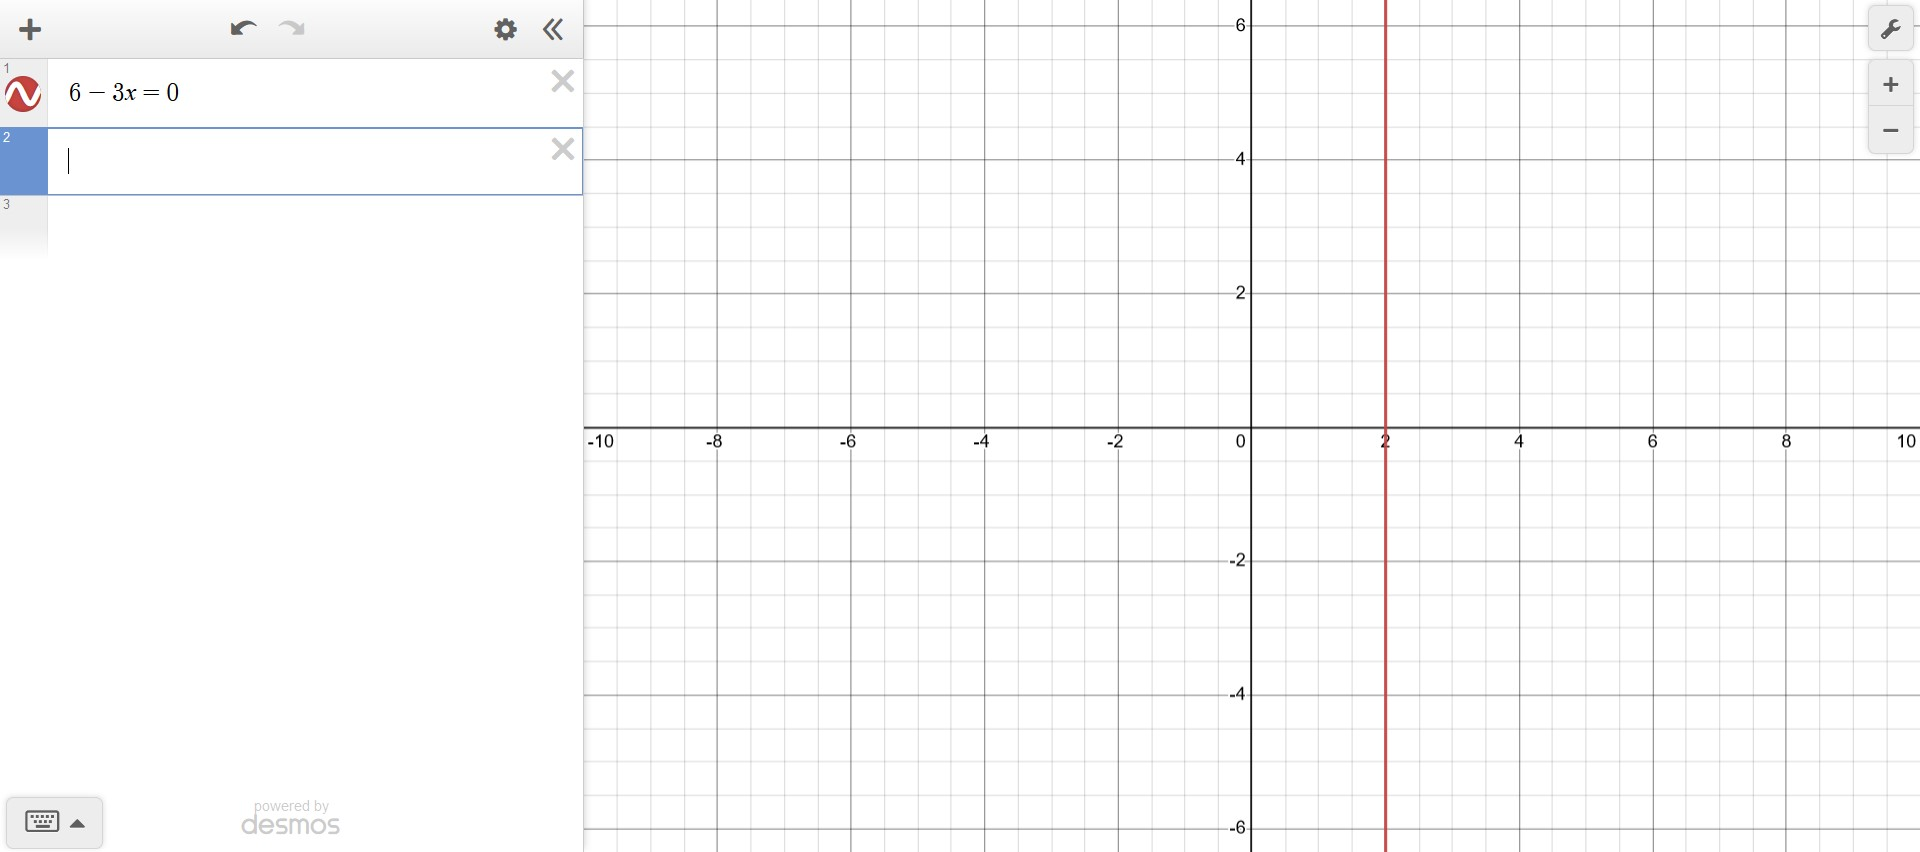
\includegraphics[width=1\textwidth]{figures/5.1.jpg}
    \caption
	{}
    \label{fig:fig1}
\end{figure}

\subsection{}
\begin{latin}
$
\theta = \begin{bmatrix}
18 \\
0 \\
6
\end{bmatrix}, \\
X = \begin{bmatrix}
1 \\
x_1\\
x_2
\end{bmatrix}, \\
g\left( z \right) = \sigma \left( z \right), \\
h\left( \theta \right) = g\left( \theta ^ t X \right),\\
\theta ^ t X = 0 \Rightarrow \\
18 + 0x_1 + 6x_2 = 0 \Rightarrow \\
x_2 = -3
$
\end{latin}
تصویر زیر مرز تصمیم را نشان می‌دهد.
\begin{figure}[H]
    \centering
    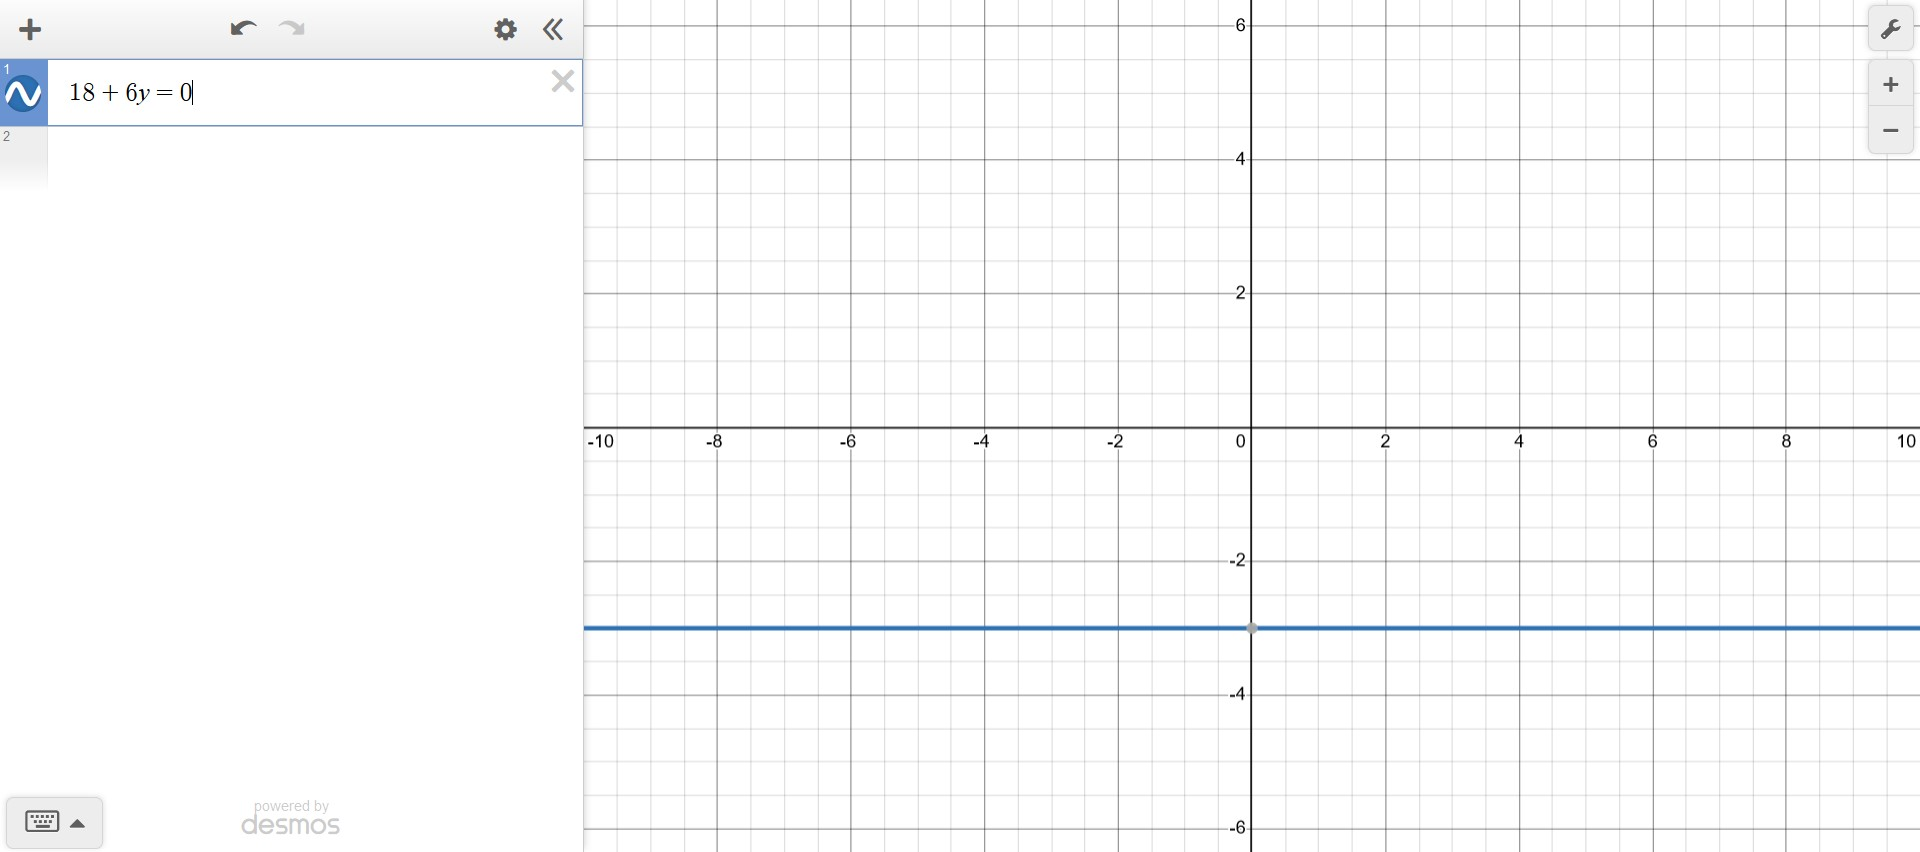
\includegraphics[width=1\textwidth]{figures/5.2.jpg}
    \caption
	{}
    \label{fig:fig1}
\end{figure}


\section{}%6
\begin{latin}
$
X = 0 \Rightarrow \sigma\left( \beta_0 + \beta_1 X \right) = \sigma\left( \beta_0 \right) = 0.5 \\ \Rightarrow \frac{1}{1 + e ^ {\beta_0}} = 0.5 \\
\Rightarrow \beta_0 = 0 \\ \\
z \ge 0\Rightarrow  \sigma\left( z \right) \ge 0.5 \\
z \le 0\Rightarrow  \sigma\left( z \right) \le 0.5 \\
$
\end{latin}
در نتیجه در مدل سبز رنگ ضریبِ $\beta_1$ منفی و در مدل سیاه رنگ ضریبِ $\beta_1$ مثبت است.


\section{}%7
\subsection{الف}
\subsubsection{}
\begin{latin}
$
z_{1_{D_{a_1} \times 1}} = W_{1_{D_{a_1} \times D_{x}}} \times x ^ {\left( i \right)}_{D_{x} \times 1} + b_{1_{D_{a_1} \times 1}}\\
z_{3_{D_{a_1} \times 1}} = W_{2_{D_{a_1} \times D_{a_1}}} \times a_{D_{a_1} \times 1} + b_{2_{D_{a_1} \times 1}}\\
$
\end{latin}
بنابراین ابعاد پارامترها به ترتیب برابر $D_{a_1} \times D_{x}$، $D_{a_1} \times 1$، $D_{a_1} \times D_{a_1}$، و $D_{a_1} \times 1$ است.
\subsubsection{}
$x^{\left( i \right)}$ها و $x^{\prime\left( i \right)}$ها در ستون‌های $X$ قرار می‌گیرند. پس ابعاد $X$ برابر است با $2D_x \times m$. همچنین $y^{\left( i \right)}$ها در ستون‌های $Y$ قرار دارند. پس ابعاد $Y$ برابر است با $1 \times m$.

\subsection{ب}
\subsubsection{}
\begin{latin}
$
\frac{\partial J}{\partial z_3}
= \frac{\partial J}{\partial L ^ {\left( i \right)}} \times \frac{\partial L ^ {\left( i \right)}}{\partial \hat{y} ^ {\left( i \right)}} \times \frac{\partial \hat{y} ^ {\left( i \right)}}{\partial z_3}
= -\frac{1}{m} \times \left( \frac{y ^ {\left( i \right)}}{\hat{y} ^ {\left( i \right)}} + \frac{1 - y ^ {\left( i \right)}}{1} \times \frac{-1}{1 - \hat{y} ^ {\left( i \right)}} \right) \times \sigma\left( z_3 \right) \left( 1 - \sigma\left( z_3 \right) \right)
= -\frac{1}{m} \times \left( \frac{y ^ {\left( i \right)}}{\hat{y} ^ {\left( i \right)}} + \frac{1 - y ^ {\left( i \right)}}{1} \times \frac{-1}{1 - \hat{y} ^ {\left( i \right)}} \right) \times \hat{y} ^ {\left( i \right)} \left( 1 - \hat{y} ^ {\left( i \right)} \right)
= \frac{\hat{y} ^ {\left( i \right)} - y ^ {\left( i \right)}}{m}
$
\end{latin}

\subsubsection{}
\begin{latin}
$ 
\frac{\partial a}{\partial z_2}
= \frac{\partial \left( a_1 - a_2 \right)}{\partial z_2}
= \frac{\partial a_1}{\partial z_2} - \frac{\partial a_2}{\partial z_2}
= - \frac{\partial a_2}{\partial z_2}
= - \frac{\partial \left( \tanh\left( z_2 \right) \right)}{\partial z_2}
= - \frac{1}{1 - z_2 ^ 2}
$
\end{latin}

\subsubsection{}
\begin{latin}
$
  \frac{\partial J}{\partial W_1}
= \frac{\partial J}{\partial L ^ {\left( i \right)}} \times \frac{\partial L ^ {\left( i \right)}}{\partial \hat{y} ^ {\left( i \right)}} \times \frac{\partial \hat{y} ^ {\left( i \right)}}{\partial z_3} \times \frac{\partial z_3}{\partial a} \times \frac{\partial \left( a_1 - a_2 \right)}{\partial W_1}
= \frac{\partial J}{\partial L ^ {\left( i \right)}} \times \frac{\partial L ^ {\left( i \right)}}{\partial \hat{y} ^ {\left( i \right)}} \times \frac{\partial \hat{y} ^ {\left( i \right)}}{\partial z_3} \times \frac{\partial z_3}{\partial a} \times \left( \frac{\partial a_1}{\partial z_1} \times \frac{\partial z_1}{\partial W_1} - \frac{\partial a_2}{\partial z_2} \times \frac{\partial z_2}{\partial W_1} \right)
= \frac{\hat{y} ^ {\left( i \right)} - y ^ {\left( i \right)}}{m} \times W_2 \times \left( \frac{1}{1-z_1 ^ 2} \times x ^ {\left( i \right)} - \frac{1}{1 - z_2 ^ 2} \times x ^ {\prime \left( i \right)} \right)
$
\end{latin}

\subsection{ج}
\subsubsection{}
\begin{latin}
$
W_1 := W_1 - \alpha \times \frac{\partial J}{\partial W_1}
= W_1 - \alpha \times \frac{\hat{y} ^ {\left( i \right)} - y ^ {\left( i \right)}}{m} \times W_2 \times \left( \frac{1}{1-z_1 ^ 2} \times x ^ {\left( i \right)} - \frac{1}{1 - z_2 ^ 2} \times x ^ {\prime \left( i \right)} \right)
$
\end{latin}

\subsubsection{}
\begin{latin}
$
b_1 := b_1 - \alpha \times \frac{\partial J}{\partial b_1}
= b_1 - \alpha \times \frac{\hat{y} ^ {\left( i \right)} - y ^ {\left( i \right)}}{m} \times W_2 \times \left( \frac{1}{1-z_1 ^ 2}  - \frac{1}{1 - z_2 ^ 2} \right)
$
\end{latin}

\subsubsection{}
\begin{latin}
$
W_2 := W_2 - \alpha \times \frac{\partial J}{\partial W_2}
= W_2 - \alpha \times \frac{\hat{y} ^ {\left( i \right)} - y ^ {\left( i \right)}}{m} \times a
$
\end{latin}

\subsubsection{}
\begin{latin}
$
b_2 := b_2 - \alpha \times \frac{\partial J}{\partial b_2}
= b_2 - \alpha \times \frac{\hat{y} ^ {\left( i \right)} - y ^ {\left( i \right)}}{m}
$
\end{latin}

\subsection{د}


%%%%%%%%%%%%%%%%%%%%%%%%%%%%%%%%%%%%%%%%%






%\begin{latin}
%\lstinputlisting{sources/p2.m}
%\end{latin}


%%%%%%%%%%%%%%%%%%%%%%%%%%%%%%%%%%%
%%%%%%%%%%%%%%%%%%%%%%%%%%%%%%%%%%%
%%%%%%%%%%%%%%%%%%%%%%%%%%%%%%%%%%%

%------------------------------------------------------------------------------------------


\subsection*{منابع}
\renewcommand{\subsection}[2]{}%
\begin{thebibliography}{99} % assumes less than 100 references
%چنانچه مرجع فارسی نیز داشته باشید باید دستور فوق را فعال کنید و مراجع فارسی خود را بعد از این دستور وارد کنید


\begin{LTRitems}

\resetlatinfont

\bibitem{b1}
\end{LTRitems}

\end{thebibliography}


\end{document}
